\chapter{Methods}
\label{chap:methods}


\section{Computaional Methods}

At the core of Morphct is the estimation of HOMO (for donor) and LUMO (acceptor). This is because 
the inputs into the marcus hopping equation are the offsets between neigboring  chromophores energy levels
determine the driving force and the the TI is estimated using a dimer method that also uses the homo level. 
With that said, quantum chemical methods give us a framework from whcih to estimate the homo/lumos. A litany of
methods that use approximations and parametrizations to transform cumbersome ab initio quantum mechanical 
calculations into efficient algorithms for determining the electronic stucuture of a given compound. Morpcht 
leverages MINDO/3, a variation of the INDO(Intermediate Neglect of Differential Overlap) method,
which is an approximation method that seeks recreate the ab initio Hartree-Fock results\cite{Thiel2014}. Results
from the this work compare well to jones2017 which implemented ZINDO/s, another semi-emperical method. The
previous version of MorphCT utilized ORCA to provide the quantum chemical approxiamtions required to implement
a hopping model of charge transport \cite{Neese2012b}. Jones2017 showed that with this you can connect MD
provided morphology to charge transport charactersitcs. A particular 
choice of method comes down to how well we can organize a workflow. 

\indent The software chosen to implement this method is
provided by pySCF (Python-based Simulations of Chemistry Framework) \cite{Sun2018a}. This framework
was chosen in the interest of reproducabilty and extensibilty. PySCF is implemented almost entirly in the Python 
language, which is becoming increasingly ubiquitious in the scientific computing community. Furthermore,
ORCA's proprietary licensing was prohibitive in the efforts to containerize MorphCT for use on cluster and for
creating reproducible results. 
Solving shrodingers equation accross tens of thousands of 
chromophores, which will be required to model an OPV material on the order of 10 nm, is untenable. Therefore
justified but drastic simplifications are necessary. 
\newline \indent
Figure blaf \ref{fig:TI} shows MorphCT calculated values the transfer integral between two thiophene
rings. Using Mbuild, a reference thiopophene is placed in the xy-plane with the y-axis running through the 
x-axis and its center mass placed at the origin. A second thiophene is instantiated in the same manner but a
combination space of allowable moves is created wherein the second thiophene can translate up to 5nm 
and rotate up to 90 degress about its x and z axis. Center-to-center distances less than 3nm are disallowed. 
This gives 4300 unique orientations show in figure blah \ref{TI}. The figure shows that, as expected,
center-to-center distance decreasing results in more orbital overlap. Also observable in the figure is that
a rotation of 90 degrees about the x axis corresponds to the sulfer of the second thiophene being oreinted
straight towards the reference thiophene corresponds to a smaller sulfer-to-sulfler distance and a greater TI. 


\begin{figure}
  \center
  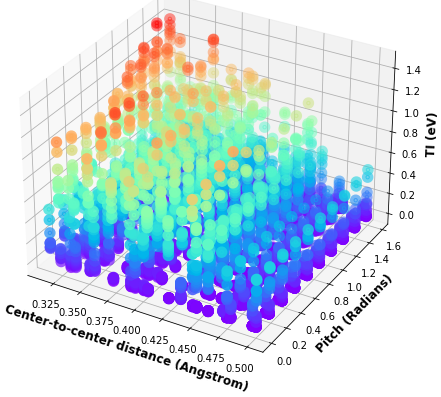
\includegraphics[width=10cm]{figures/transfer_integral_plot.png}
  \caption{Thiophene Transfer Integrals}
  \label{fig:TI}
\end{figure}

\section{\nobreak kmc analysis}
Taking a charge to be a quasi-particle inserted into a MD generated morpholgy, a KMC
simulation can be run on the bases of Marcus rates obtained from QCC.
The KMC algorithm allows an explicit calculation of the MSD accross a large number of 
particles in the system. Repeating along relevant time scales for 
charge transfer, knowing that MSD scales linearly with time, the slope of this relationship
can be estimated and related to to the 3D diffusion coeffiecient. Using the Einstien relation, 
the groundwork for which Einstein derived in his doctoral dissertaion, finally the zero-field
mobility can be obtained. 


%%% Local Variables: 
%%% mode: latex
%%% TeX-master: "BSUmain"
%%% End: 
